\documentclass[11pt,letterpaper]{article}
\usepackage[lmargin=1in,rmargin=1in,bmargin=1in,tmargin=1in]{geometry}
\usepackage{style/quiz}
\usepackage{style/commands}

% -------------------
% Content
% -------------------
\begin{document}
\thispagestyle{title}

% Quiz 1
\quizsol \textit{True/False}: Ethan is saving for a new car. The car he is saving for costs \$9,800. Over the next two months, the cost of the car rises by 8\% each month. Therefore, the car now costs 16\% more and thus costs $\$9800(0.16)= \$1568$ more than it did when he started saving. \pspace

\sol The statement is \textit{false}. Repeated percent increase/decrease are not additive; that is, applying a $P$\% increase/decrease to a number $X$ a total of $n$ times is not the same thing as finding a $nP$\% increase/decrease. In this case, raising the price 8\% twice is not the same thing as raising the price by 16\%. The price increase after the first month is $\$9800(0.08)= \$784$. The new price is then $\$9800 + \$784= \$10584$. The price increase the second month is then $\$10584(0.08)= \$846.72$. The final price is then $\$10584 + \$846.72= \$11430.70$. [Note: One could compute this immediately via $\$9800(1.08)^2= \$9800(1.1664)= \$11430.70$.] But then the car costs $\$11430.70 - \$9800= \$1630.72$ more than when he bought it. Alternatively, we know that the original price was $\$9800$. After increasing the price twice by 8\%, the final price will be $\$9800(1.08)^2= \$9800(1.1664)$. We can recognize this as a 16.64\% increase from the original price. But this is $\$9800(0.1664)= \$1630.72$ increase in price. \pvspace{1.3cm}



% Quiz 2
\quizsol \textit{True/False}: Ellen has been hired as a financial analyst at a company. The previous analyst modeled the cost of producing one of their products as $C(q)= 43.27q + 13296$. Therefore, Ellen can deduce that the model predicted that the production cost of each item was $\$43.27$ and the fixed costs were $\$13296$. \pspace

\sol The statement is \textit{true}. We know that the cost of production per unit (at a production level of $q$~items) is the rate of change of $C(q)$. Because $C(q)$ is linear, this is the slope of $C(q)$. The slope of $C(q)$ is $43.27$. Therefore, the item costs $\$43.27$ per item to produce, as claimed. Finally, we know that the fixed costs are the costs regardless the level of production. But then the fixed costs will be the costs associated with producing 0~units. This is $C(0)= 43.27(0) + 13296= 13296$. Therefore, the fixed costs are \$13,296, as claimed. \pvspace{1.3cm}



% Quiz 3
\quizsol \textit{True/False}: If the CPI last year was \$248.110 and this year it is \$251.608, then the inflation rate from last year to this year was 1.41\%. Moreover, if the inflation rate stays constant, in 5~years, goods will cost approximately 7.25\% more. \pspace

\sol The statement is \textit{true}. We have $\dfrac{251.608}{248.110}= 1.014099= 1 + 0.014099$. Therefore, prices have increased by $1.4099\%$. Then if a good/service costs $\$P$ now and the rate of inflation stays constant in 5~years it will cost $P(1 + 0.014099)^5= P(1.014099)^5= P(1.07251)= P(1 + 0.07251)$. But then prices are $7.251\%$ more expensive in 5~years. \pvspace{1.3cm}



% Quiz 4
\quizsol \textit{True/False}: The expression $8000 \left(1 + \dfrac{0.051}{4} \right)^{12}$ could represent the amount of money in a savings account earning 5.1\% annual interest, compounded quarterly after 12~years if the savings account initially had \$8,000 deposited into it. \pspace

\sol The statement is \textit{false}. We know that if an initial amount $P$ accruing interest at an annual rate of $r$\% per year, compounded $k$ times per year for $t$ years, the final amount is given by $P \left(1 + \dfrac{r}{k} \right)^{kt}$. Writing the function above in this form, we have\dots
	\[
	8000 \left(1 + \dfrac{0.051}{4} \right)^{12}= 8000 \left(1 + \dfrac{0.051}{4} \right)^{4 \cdot 3}
	\]
Then here we have $P= \$8000$, $r= 0.051$ (a 5.1\% annual interest rate), $k= 4$ (compounded quarterly), and $t= 3$. Therefore, this could represent the final amount of an initial investment of \$8,000 at an annual interest rate of 5.1\%, compounded quarterly, invested for 3~years. \pvspace{1.5cm}



% Quiz 5
\quizsol \textit{True/False}: Terry has taken out a 5~year loan for 8.3\% annual interest, compounded monthly. The bank requires him to make equal monthly payments on the first of the month. Terry's loan is an example of a simple annuity. \pspace

\sol The statement is \textit{false}. Because the number of payments each year matches the number of compounds each year, this is a simple annuity. Because payments are due at the start of each pay period, this is an annuity due. Therefore, this is a simple annuity due. \pvspace{1.5cm}



% Quiz 6
\quizsol \textit{True/False}: Ann Euity has taken out a 30~year, fixed rate mortgage for a new \$250,000 home. The mortgage has a yearly annual interest of 6.87\%, compounded monthly. Her beginning of the month payments are \$1,632.14. After making her first payment, she owes $\$250000 - \$1632.14= \$248367.86$ on her mortgage. \pspace

\sol The statement is \textit{false}. This is an amortized loan. In an amortized loan, the payment amount is fixed. But each payment goes towards paying off the loan \textit{and} the interest owed during that pay period simultaneously. Therefore, some portion of the initial payment should have gone towards paying off the interest due on the remaining loan amount for that month. But then the amount owed cannot decrease by the full amount of the monthly payment. The amount that the loan would decrease by would be the payment against the principal for that month, which is\dots
	\[
	\begin{aligned}
	\text{PAP}&= R \left( \ddot{a}_{\actuarialangle{n - m + 1\,}\, i} - \ddot{a}_{\actuarialangle{n - m\,}\, i} \right) \\[0.3cm]
	&=  1632.14 \left( \ddot{a}_{\actuarialangle{360 - 1 + 1\,}\, 0.005725} - \ddot{a}_{\actuarialangle{360 - 1\,}\, 0.005724} \right) \\[0.3cm]
	&= 1632.14 (153.1728651 - 153.0440548) \\[0.3cm]
	&= \$210.24
	\end{aligned}
	\] 



\newpage



% Quiz 7
\quizsol \textit{True/False}: If $A$ and $B$ are disjoint events with $P(A)= \frac{1}{3}$ and $P(B)= \frac{4}{5}$, then $P(A \text{ and } B)= P(A) \cdot P(B)= \frac{1}{3} \cdot \frac{4}{5}= \frac{4}{15}$. \pspace

\sol The statement is \textit{false}. Recall that $P(A \text{ and } B)= P(A) \cdot P(B)$ if and only if the events $A$ and $B$ are independent, i.e. the occurrence or non-occurrence one does not change the probability that the other occurs. Recall that disjoint events can \textit{never} be independent. Disjoint events cannot occur at the same time. Therefore, if one event occurs, the other does not. Hence, disjoint events cannot be independent. Because $A$ and $B$ cannot occur at the same time, it is clear that $P(A \text{ and } B)= 0$. \pvspace{1.3cm}



% Quiz 8
\quizsol \textit{True/False}: If $A$ and $B$ are independent events with $P(A)= 0.40$ and $P(B)= 0.50$, then $P(A \text{ or } B)= 0.70$. \pspace

\sol The statement is \textit{true}. Recall that\dots
	\[
	P(A \text{ or } B)= P(A) + P(B) - P(A \text{ and } B)
	\]
We know $P(A \text{ and } B)= P(A) \cdot P(B)$ if and only if the events $A$ and $B$ are independent, i.e. the occurrence or non-occurrence one does not change the probability that the other occurs. Because $A$ and $B$ are independent, we know that $P(A \text{ and } B)= P(A) \cdot P(B)= 0.40 \cdot 0.50= 0.20$. But then we have\dots
	\[
	P(A \text{ or } B)= P(A) + P(B) - P(A \text{ and } B)= 0.40 + 0.50 - 0.20= 0.70
	\] \pvspace{1.3cm}



% Quiz 9
\quizsol \textit{True/False}: Fernando is playing a carnival game. After paying \$2, you spin a giant wheel and if it lands in the green region, you win \$20. However, the rest of the wheel is red and if you land in this region, you must pay \$1. There is only a 10\% chance you land in the green region. Fernando claims that playing this game, in the `long-run average', you make money playing this game. \pspace

\sol The statement is \textit{false}. Because the wheel consists only of a red and green region and the probability of spinning green is 10\%, there is a 90\% chance that one spins red. If you spin green, you win \$20 having paid \$2 for a net gain of \$18. If you spin red, you lose \$1 having paid \$2 for a net loss of \$3. We can create a table of the possibilities for a spin, the spin's probability, and the net gain/loss from the spin. 
	\begin{table}[!ht]
	\centering
	\begin{tabular}{|l|c|c|} \hline
	& Green & Red \\ \hline
	Probability & 0.10 & 0.90 \\ \hline
	Amount & \$18 & $-$\$3 \\ \hline
	\end{tabular}
	\end{table}
We can then compute the expected value for this game:
	\[
	EX= \sum x P(X= x)= \$18(0.10) + (-\$3)(0.90)= -\$0.90
	\]
Therefore, in the `long run', one loses an average of \$0.90 per game. Because this expected value is negative, in the `long run', you lose money playing this game. 



\newpage



% Quiz 10
\quizsol \textit{True/False}: If you fit a linear regression to a set of data and $R^2= 1$ for the regression, then the data was perfectly linear. \pspace

\sol The statement is \textit{true}. The coefficient of determination, $R^2$, is 1 if and only if the data is perfectly linear. In terms of the (Pearson) correlation coefficient, the data is perfectly linear if and only if $R= 1$ or $R= -1$. If $R= 1$, the data is perfectly linear and positively correlated. If $R= -1$, the data is perfectly linear and negatively correlated. \pvspace{1.3cm}



% Quiz 11
\quizsol \textit{True/False}: The larger the value of $|z_x|$ is in a normal distribution, the more `unusual' the value $x$. \pspace

\sol The statement is \textit{true}. For a normal distribution, we know that $z_x$ is the number of standard deviations $x$ is above or below the mean. Therefore, $|z_x|$ is the number of standard deviations $x$ is from the mean. The farther that $x$ is from the mean in a normal distribution, the less probable that one `sees' a value farther than $x$ from the mean. But then $x$ is more `unusual' compared to the majority of other values in the distribution. \pvspace{1.3cm} 



% Quiz 12
\quizsol \textit{True/False}: For the distribution $N(100, 10)$, we know $P(X \leq 85)= P(X \geq 115)$. \pspace

\sol The statement is \textit{true}. Observe that $85$ is 1.5 standard deviations (that is $15$) below from the mean of $100$. Observe that also $115$ is also 1.5 standard deviations (that is $15$) above the mean of $100$. Because the normal distribution is symmetric, the probability of being less than 1.5 standard deviations below the mean must be the same as the probability of being 1.5 standard deviations above the mean. Alternatively, we can compute this directly:
	\[
	\begin{aligned}
	z_{85}&= \dfrac{85 - 100}{10}= \dfrac{-15}{10}= -1.5 \squiggle 0.0668
	z_{115}&= \dfrac{115 - 100}{10}= \dfrac{15}{10}= 1.5 \squiggle 0.9332
	\end{aligned}
	\]
But then we have $P(X \leq 85)= 0.0668$ and $P(X \geq 115)= 1 - P(X \leq 115)= 1 - 0.9332= 0.0668$. \pvspace{1.3cm}



% Quiz 13
\quizsol \textit{True/False}: For a fixed probability $p$, as the number of observations $n$ gets larger and larger, the distribution $B(n, p)$ `looks' more like a normal distribution. \pspace

\sol The statement is \textit{true}. For any fixed probability $p$, the larger the value of $n$, the closer the binomial distribution `resembles' a normal distribution. This is precisely what allows one to approximate a binomial distribution with a normal distribution for sufficiently large $n$. Below we illustrate this by plotting the binomial distribution $B(n, 0.50)$ for $n= 10$, $20$, and $50$ (illustrated in blue, yellow, and green, respectively). 
	\begin{figure}[!ht]
	\centering
	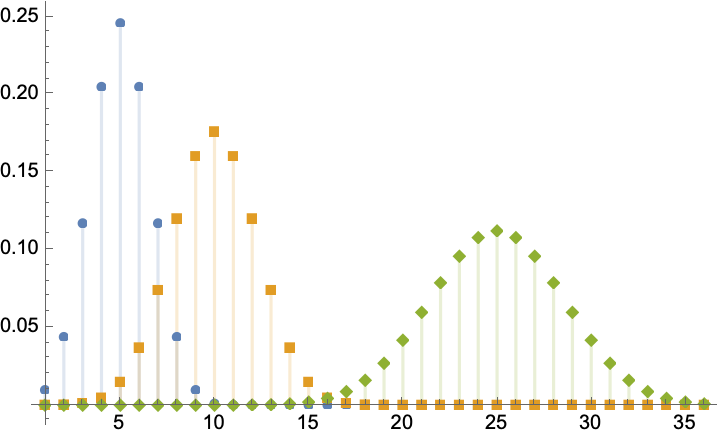
\includegraphics[width= 0.22\textwidth]{binomial.png}
	\end{figure}



% Quiz 14
\quizsol \textit{True/False}: The larger the sample sized used in creating a confidence interval, the smaller the size of that confidence interval. \pspace

\sol The statement is \textit{true}. This is intuitively true via the following argumentation: the larger the sample, the more likely that sample is to `resemble' the entire population. Then the sample mean should be `close' to the underlying population mean so that ones uncertainty in this estimation should be low. This results in a smaller confidence interval. To see this concretely, recall that the length of a confidence interval is twice the margin of error. The margin of error is $z^* \, \frac{\sigma}{\sqrt{n}}$. The larger the value of $n$, the larger the value of $\sqrt{n}$. But this in turn makes $\frac{1}{\sqrt{n}}$ smaller so that $z^* \, \frac{\sigma}{\sqrt{n}}$, i.e. the margin of error, smaller. This results in a smaller confidence interval. \pvspace{1.3cm}



% Quiz 15
\quizsol \textit{True/False}: The normal distribution is a continuous distribution. Because the binomial distribution is a discrete distribution, the normal distribution cannot be used to approximate binomial probabilities. \pspace

\sol The statement is \textit{false}. For any fixed probability $p$, the larger the value of $n$, the closer the binomial distribution `resembles' a normal distribution. This is precisely what allows one to approximate a binomial distribution with a normal distribution for sufficiently large $n$. Below we illustrate this by plotting the binomial distribution $B(n, 0.50)$ for $n= 10$, $20$, and $50$ (illustrated in blue, yellow, and green, respectively). 
	\begin{figure}[!ht]
	\centering
	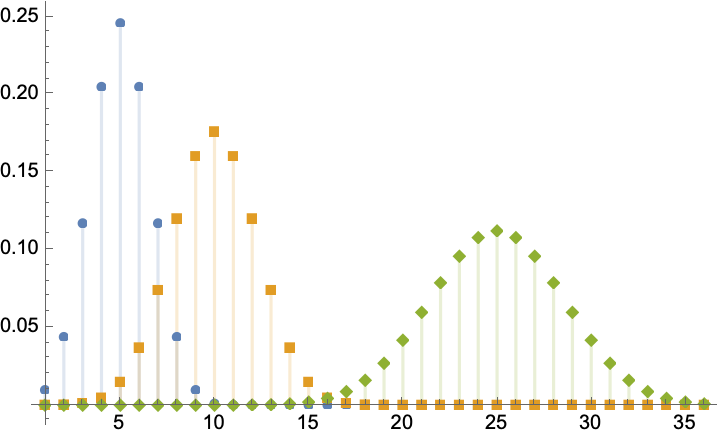
\includegraphics[width= 0.22\textwidth]{binomial.png}
	\end{figure}



% Quiz 16

If $\mathbf{u}= (2 \;\;-1\;\;0)$ and $\mathbf{v}= (-3\;\;-6\;\;5)$, then $\mathbf{u} \cdot \mathbf{v}= (-6\;\;6\;\;0)$. 






\newpage


If $A$ is a $6 \times 9$ matrix and $B$ is a $6 \times 9$ matrix, then the product $AB$ is defined and is a $6 \times 9$ matrix. 

The following matrix in RREF could represent a system of three equations in three unknowns with solution $x_1= 1$, $x_2= 2$, and $x_3= 3$,
	\[
	\begin{pmatrix}
	1 & 0 & 0 & 1 \\
	0 & 1 & 0 & 2 \\
	0 & 0 & 1 & 3 
	\end{pmatrix}
	\]


















































\end{document}